%\url{http://commons.oreilly.com/wiki/index.php/SVG_Essentials/Transforming_the_Coordinate_System}


\section{Animácie }

TUTO PRIBUDNE TABULKA TOHO CO SA DA REALIZAT CEZ SVG A CO CEZ SNAP.SVG.
bud to bude na konci ako zhrnutie alebo na zacia
\url{http://www.w3.org/1999/07/30/WD-SVG-19990730/animate.html} - zoznam dostupnych SVG animacii, prejdi si to prosim a skus najst analogie v snap.js kniznici. animateFlipbook nie je moc dolezita, ale ostatne mozes dat do bakalarky aj s prikladmi.
\begin{table}[H]
	
	\begin{center}
		\begin{tabular}{|p{3cm}|p{3cm}|p{3cm}|p{3cm}|}
			\hline \textbf{Animacia} & \textbf{SVG akcia} & \textbf{JavaScript akcia} & \textbf{Popis} \\ 
			\hline Animácia &  &  &  \\ 
			\hline Nastavenie farby &  &  &  \\ 
			\hline Transformácia &  &  &  \\ 
			\hline Skryvanie  &  & attr({visibility: true}) &  \\ 
			\hline Atributy farby & animateColor  & attr({fill: farba}) &  \\ 
			\hline  &  &  &  \\ 
				\hline Nastavenie atributov & set element & metoda attr &  \\ 
				\hline zmena farby & animateColor element & attr(fill: farba) &  \\ 
				\hline animovanie transformacie & animateTransform element & transform() &  \\ 
				\hline  & animateMotion element &  &  zoznam atributov pridate este\\ 
				\hline  &  &  &  \\ 
				\hline  &  &  &  \\ 
				\hline 
		
			\hline 
		\end{tabular} 
	\end{center}
	
	\caption{Mapovacia tabuľka}
	\label{haha2}
\end{table}

 V SVG SMIL animacia používa tieto elementy:
 \begin{itemize}
 	 \item The ‘animate’ element
 \item The ‘set’ element
 \item  The ‘animateMotion’ element
  \item The ‘animateTransform’ element
\end{itemize}



O čom bude táto časť: 
\begin{itemize}
	\item Animácia metód a jednoduchých atribútov animácie TODO ZMENA FARBY INDIKATORA 
	\item Animovanie path TODO KAPITOLA O NADRZI
	\item Easing využívajúc kubickú Bézierovú syntax
	\item Animácie transformácie TODO KAPITOLA ROTOR
	\item Animácie využívajúce spoločné atribúty a animácie popri path TODO MAPA CESTY
\end{itemize}

\section{Animacia - Element.animate(...)}
Snap.animation = function (attr, ms, easing, callback) 
\begin{itemize}
\item	- attr (object) atribúty finalného produktu
\item	- duration (number) trvanie animácie v milisekundách , 
\item - easing (function) vid tabluka, alebo kapitola o tom 	funkcie  @mina 
\item funkcia, ktorá sa vykoná po skončení animácii
\end{itemize}



\subsection{Animácia atribútov}
TODO NAPR ZMENA FARBY INDIKATORA TOKU VODY

tabulka ake atributy sa daju menit
napr
\begin{itemize}
	\item visibility: / attr({visibility: true})
	\item okrajov: pozri tabulku c. \ref{parametre:styl}
	\item farby: pozri tabulku 
	\item textu: tabulka \ref{tab:text}
	\item tvarov: tabulka \ref{parametre:tvar}
\end{itemize}



\subsection{Animácia elementov, path}
TODO NAPR ANIMOVANIE ZMENY PRITOKU VODY DO NADRZE
\subsection{Animation easing}
Easing describes how the value of an attribute varies with regard to time. By default,
the value of an attribute changes consistently—that is, linearly—over the course of
an animation but by specifying a particular easing type, we can change the way in
which the attribute is animated. Consider the following graph that demonstrates
three of the available easing types\ref{fig:easing}:
\cite{Dawber}[p~70]

\begin{figure}[H]
\centering
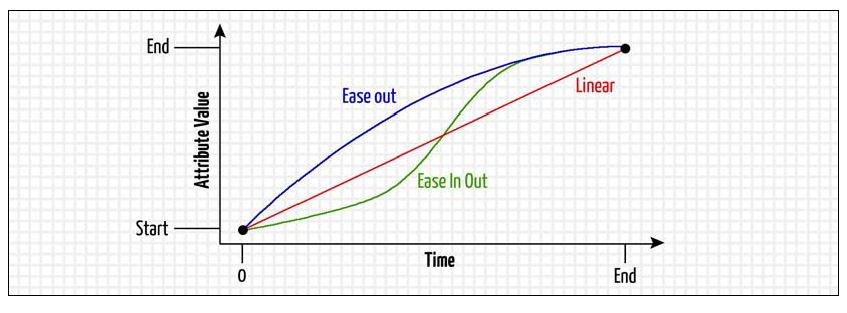
\includegraphics[width=0.7\linewidth]{obrazky/easing}
\caption{Graf troch easing typov}
\label{fig:easing}
\end{figure}


For each easing type, the rate at which the attribute changes varies along the graph in
the time axis. Each easing type can be described as such:
\begin{itemize}
	

\item Linear: The value varies consistently from its start value to its end value over
the course of the animation
\item Ease Out: The value increases quickly towards its end point before slowing
down towards the end of the animation
\item Ease In Out: The value decreases slowly at first and then increases quickly
before finally slowing down to its end point towards the end of the animation
\end{itemize}




\subsection{Animácia transformácií}
TODO ASI TEN VENTIL BY BOLO VHODNE ZANIMOVAT A TRANSFORMOVAT

\subsection{Animacia vyuzivajuca vlastne atributy}

\subsection{Animacia podla path}
toto uz v prikladoch mam ako mapu TODO /
todo urobit pri nadrzi 

\subsection{Pausing a resuming animation}

















\section {Práca s Existujúcimi SVG}

Táto sekcia bude o práci s existujúcim .svg súborom cez: 
\begin{itemize}
	\item Inkscape vektorový grafický editor
	\item Manuál na vyšetrenie SVG paths
	\item Príklad zistenia SVG id
\end{itemize}


\section{Inkscape}
\section{Definovanie id SVG}
\section{Zoznam id SVG atributov vyuzite v priklade}